\section{Counter-Strike}

\begin{figure}[htbp]
\begin{center}
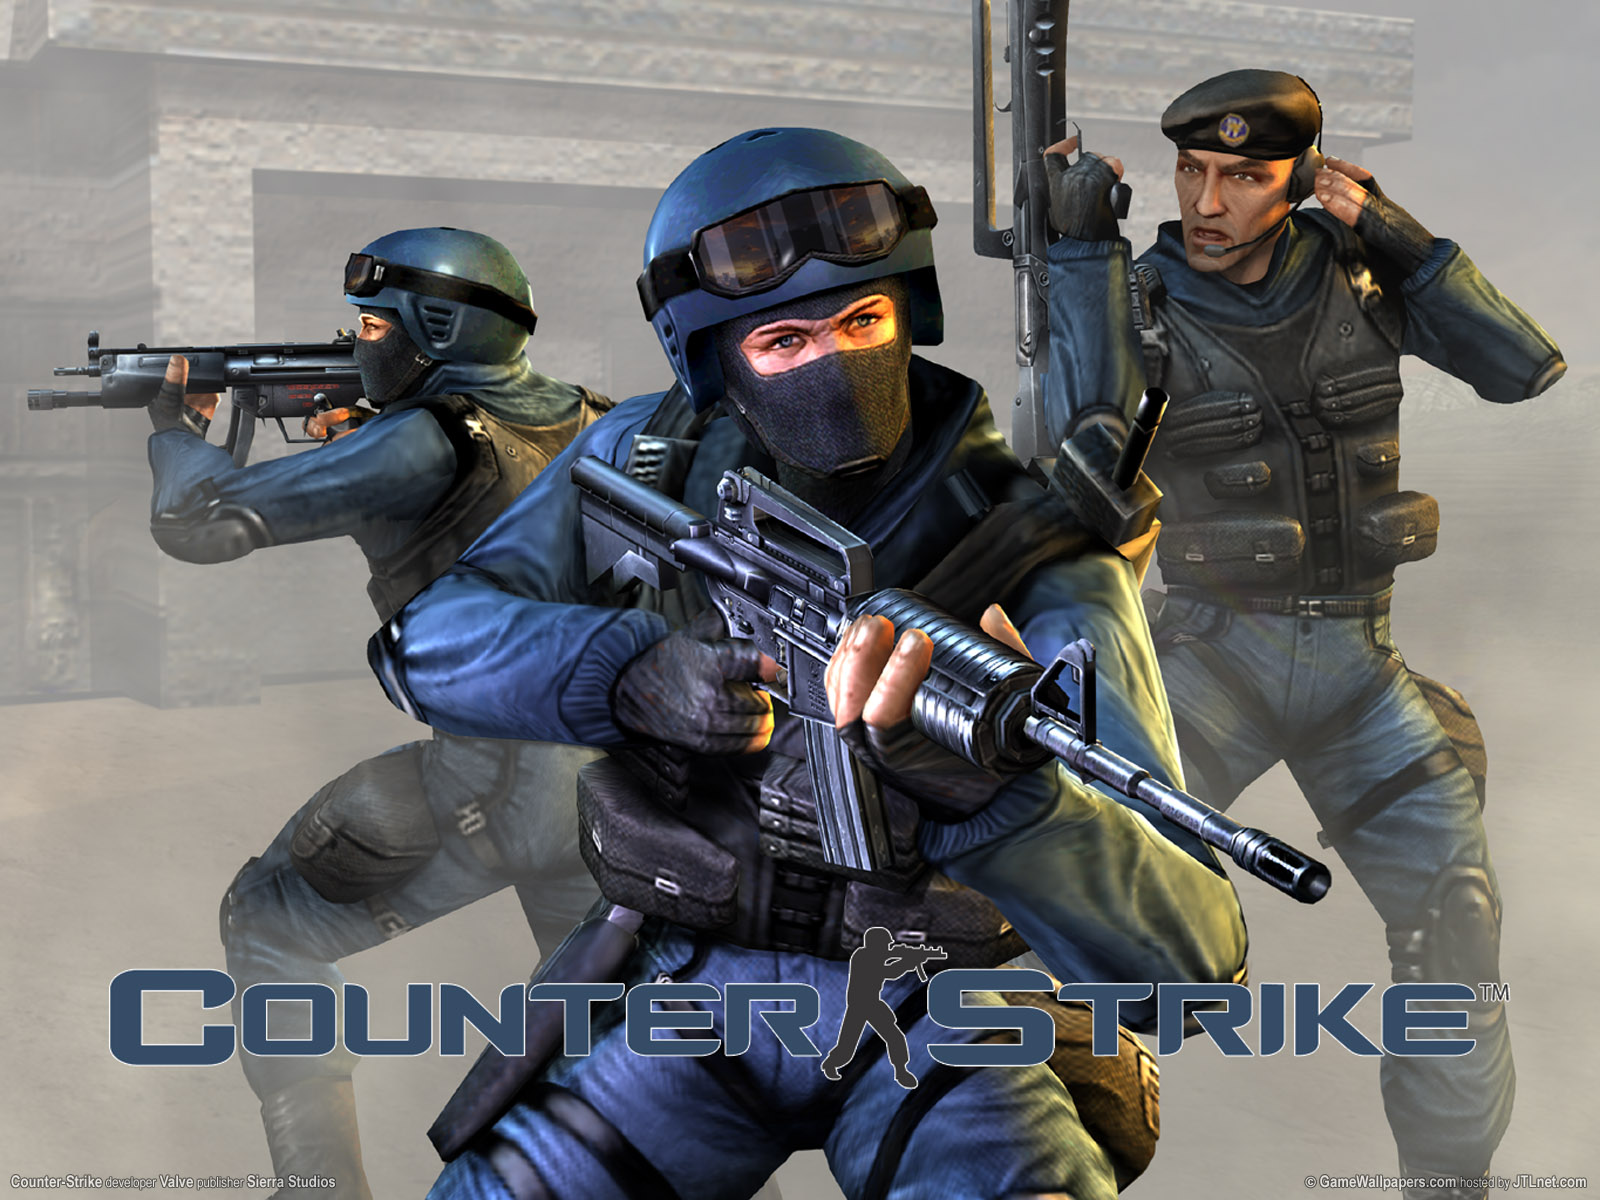
\includegraphics[width=.60\textwidth]{./imagenes/CounterStrike.jpg}
\caption{Counter-Strike}
\label{Counter-Strike}
\end{center}
\end{figure}
Counter-Strike\footnote{\url{http://http://store.steampowered.com/css/}} es un juego de tipo multijugador. La acción de Counter-Strike se desarrolla en rondas de una duración elegida por el que las crea, en la cual un equipo de terroristas se enfrenta a un equipo de antiterrorista. El equipo victorioso es el que cumpla todos sus objetivos de victoria, de situación o la eliminación de todos los jugadores del otro equipo. Si al final de la ronda no hay victoria directa de uno de los dos equipos, el equipo que no realizó sus objetivos pierde por eliminación.

\subsubsection{¿Por qué es uno de mis juegos favoritos?}
\begin{itemize}
\item[Edwin Hermenejildo] Counter-Strike Agrupa varios aspectos del espíritu deportista: trabajo de equipo, competencia, igualdad de oportunidades y con su éxito es lógico que el juego haya dado a un gran número de jugadores el deseo de competir.
Todos los jugadores comienzan con la misma cantidad de puntos de vida y la cantidad de puntos de armadura que consiguieron conservar durante la ronda anterior siempre y cuando no compren una nueva. Cuando los daños son causados por los disparos de sus adversarios o sus compañeros -si hay fuego amigo- (los compañeros causan menos daño, pero pueden matar igualmente), así como por una caída violenta los puntos de vida del jugador disminuyen. Los disparos se pueden localizar en diferentes partes del cuerpo (brazo derecho e izquierdo, pierna derecha e izquierda, torso, y cabeza), y causan más o menos daños según el lugar afectado, sabiendo que un disparo en la cabeza o headshot es a menudo mortal. La pérdida de puntos de vida solo causa una pequeña disminución en los movimientos del terrorista o antiterrorista que haya recibido el daño. Cuando la totalidad de los puntos de vida se terminan, el jugador muere.
\end{itemize}
